\documentclass{article}

%%% Packages %%%

% Graphics
\usepackage{graphicx}
\usepackage[caption=false,font=footnotesize]{subfig}

% Formatting
\usepackage{color}
\usepackage{amsmath}
\usepackage{amssymb}
\usepackage{amsfonts}
\usepackage{bbm}
\usepackage[T1]{fontenc}

\usepackage{garamond}


% Environments
\usepackage{IEEEtrantools}
\usepackage{algorithm}
\usepackage{algorithmic}

% References
\usepackage{natbib}

% Macro
\usepackage{etoolbox}


%%% Graphics %%%
\graphicspath{{figures/}}


%%% Macros %%%
%%% MACROS FOR MATHEMATICAL NOTATION IN BCG HEARTBEAT INFERENCE PAPER %%%

% Functions and operators
\newcommand{\half}{\frac{1}{2}}                                 % Half
\DeclareMathOperator{\sinc}{sinc}                               % Sinc
\DeclareMathOperator{\trace}{Tr}                                % Trace
\newcommand{\expect}[1]{\mathbb{E}_{#1}}                        % Expectation
\newcommand{\variance}[1]{\mathbb{V}_{#1}}                      % Variance
\newcommand{\magdet}[1]{\left|\left| #1 \right|\right|}         % Magnitude of the determinant
\newcommand{\indic}[1]{\mathbbm{1}_{#1}}                        % Indicator function
\newcommand{\bigo}[1]{\mathcal{O}\left({#1}\right)}             % Big O
\newcommand{\mhaccept}{\alpha}                                  % Metropolis-Hastings acceptance probability

% Density families
\newcommand{\normalden}[3]{\mathcal{N}\left(#1\left|#2,#3\right.\right)}    % Normal density
\newcommand{\gammaden}[3]{\mathcal{G}\left(#1\left|#2,#3\right.\right)}            % Gamma density
\newcommand{\studenttden}[4]{\mathcal{ST}\left(#1|#2,#3,#4\right)}          % Student-t density

% Particle shizzle
\newcommand{\numpart}{N_P}                      % Number of particles
\newcommand{\pss}[2][]{^{(#2)#1}}               % Particle superscript
\newcommand{\pw}[1]{w_{#1}}                     % Particle weight
\newcommand{\predpw}[1]{\hat{w}_{#1}}           % Predictive particle weight
\newcommand{\npw}[1]{\bar{w}_{#1}}              % Normalised particle weight
\newcommand{\naw}[1]{\bar{v}_{#1}}              % Normalised auxiliary weight
\newcommand{\anc}[1]{a_{#1}}                    % Particle ancestor

% Time variables
\newcommand{\ti}{n}                             % Observation/time indexing
\newcommand{\timax}{N}                          % Maximum Observation/time index
\newcommand{\ot}[1]{t_{#1}}                     % Observation time
\newcommand{\ct}{t}                             % Continuous time

% Latent state and observations
\newcommand{\cls}[1]{x(#1)}                     % Continuous time latent state
\newcommand{\ob}[1]{y_{#1}}                     % Observation

% Changepoints
\newcommand{\sqi}{s}                                                        % Sequence index
\newcommand{\cpi}{k}                                                        % Changepoint indexing
\newcommand{\dmrcpi}[2][]{\ifstrempty{#1}{K_{#2}}{{K_{#2}^{[#1]}}}}         % Most recent changepoint index preceeding an observation time
\newcommand{\cmrcpi}[2][]{\ifstrempty{#1}{K(#2)}{{K^{[#1]}(#2)}}}           % Most recent changepoint index preceeding a continuous time
\newcommand{\cpt}[2][]{\ifstrempty{#1}{\tau_{#2}}{{\tau_{#2}^{[#1]}}}}      % Changepoint time
\newcommand{\cpp}[2][]{\ifstrempty{#1}{u_{#2}}{{u_{#2}^{[#1]}}}}            % Changepoint parameter
\newcommand{\cplp}[2][]{\ifstrempty{#1}{z_{#2}}{{z_{#2}^{[#1]}}}}           % Changepoint linear parameter
\newcommand{\cp}[2][]{\ifstrempty{#1}{\theta_{#2}}{\theta_{#1 || #2}}}      % Changepoint set

% Extra changepoint things for algorithms
\newcommand{\augcp}[2][]{\ifstrempty{#1}{\theta_{#2}^*}{\theta_{#1 || #2}^*}}                   % Augmented changepoint set
\newcommand{\diffcpi}[1]{\Delta K^{[#1]}}                                                       % Number of changepoints in the window
\newcommand{\intcpt}[2][]{\ifstrempty{#1}{\tau_{#2}^*}{{\tau_{#2}^{*[#1]}}}}                    % Temporary Intermediate changepoint time
\newcommand{\repcpt}[2][]{\ifstrempty{#1}{\tilde{\tau}_{#2}}{{\tilde{\tau}_{#2}^{[#1]}}}}       % Replacement changepoint time
\newcommand{\repintcpt}[2][]{\ifstrempty{#1}{\tilde{\tau}_{#2}^*}{{\tilde{\tau}_{#2}^{*[#1]}}}} % Replacement temporary Intermediate changepoint time
\newcommand{\repcp}[2][]{\ifstrempty{#1}{\tilde{\theta}_{#2}}{\tilde{\theta}_{#1 || #2}}}       % Changepoint set replacement
\newcommand{\repaugcp}[2][]{\ifstrempty{#1}{\tilde{\theta}_{#2}^*}{\tilde{\theta}_{#1 || #2}^*}}       % Changepoint set replacement


% State and observation dynamics
\newcommand{\transfun}[1][]{\ifstrempty{#1}{F}{F^{[#1]}}}               % Deterministic transition function
\newcommand{\cplppriormn}[1][]{\ifstrempty{#1}{m_0}{m_0^{[#1]}}}        % Prior mean for changepoint linear parameter
\newcommand{\cplppriorvr}[1][]{\ifstrempty{#1}{P_0}{P_0^{[#1]}}}        % Prior variance for changepoint linear parameter
\newcommand{\cplptransmat}[2][]{\ifstrempty{#1}{A_{#2}}{A_{#2}^{[#1]}}} % Parameter transition matrix for Rao-Blackwellisable models
\newcommand{\cplptranscov}[2][]{\ifstrempty{#1}{Q_{#2}}{Q_{#2}^{[#1]}}} % Parameter covariance matrix for Rao-Blackwellisable models
\newcommand{\obsmat}[1]{H_{#1}}                                         % Observation matrix
\newcommand{\obscov}[1]{R_{#1}}                                         % Observation covariance matrix

% Composites for Kalman filtering and likelihood evaluations
\newcommand{\cplpcat}[1]{\bar{z}_{#1}}              % Concatenated latest linear parameters
\newcommand{\transfuncat}{\bar{F}}
\newcommand{\cplptransmatcat}[1][]{\ifstrempty{#1}{\bar{A}}{\bar{A}^{[#1]}}}
\newcommand{\cplptranscovcat}[1][]{\ifstrempty{#1}{\bar{Q}}{\bar{Q}^{[#1]}}}

\newcommand{\cplpwin}{\mathbf{z}}                   % Concatenated linear parameters for the whole window
\newcommand{\obwin}{\mathbf{y}}
\newcommand{\transfunwin}[1][]{\ifstrempty{#1}{\mathbf{F}}{\mathbf{F}^{[#1]}}}
\newcommand{\obsmatwin}{\mathbf{H}}
\newcommand{\obscovwin}{\mathbf{R}}
\newcommand{\cplptransmatwin}[2][]{\ifstrempty{#1}{\mathbf{A}_{#2}}{\mathbf{A}_{#2}^{[#1]}}}
\newcommand{\cplptranscovwin}[2][]{\ifstrempty{#1}{\mathbf{Q}_{#2}}{\mathbf{Q}_{#2}^{[#1]}}}
\newcommand{\cplpupdmnwin}{\mathbf{\mu}}
\newcommand{\cplpupdvrwin}{\mathbf{\Sigma}}
\newcommand{\cplppredmnwin}{\hat{\mathbf{m}}}
\newcommand{\cplppredvrwin}{\hat{\mathbf{P}}}


% Probabilities
\newcommand{\prob}{P}                                                                                       % Probability
\newcommand{\survfunc}[4][1]{\ifstrempty{#1}{S\left(#2,#3,#4\right)}{S^{[#1]}\left(#2,#3,#4\right)}}        % Survivor function
\newcommand{\transden}[2][]{\ifstrempty{#1}{p_{#2}}{p^{[#1]}_{#2}}}                                         % Transition density
\newcommand{\impden}[2]{q_{#1 || #2}}           % Changepoint importance density
\newcommand{\artden}[2]{\rho_{#1 || #2}}        % Changepoint artificial density
\newcommand{\adjden}{\varphi}                   % Changepoint time ``adjustment'' density
\newcommand{\intden}[1]{\psi_{#1}}              % Intermediate changepoint artificial target density
\newcommand{\lhood}{p_{y}}                      % Likelihood
\newcommand{\loglhood}{L_{y}}                   % Log-likelihood
\newcommand{\contlhood}{\phi}                   % Contracted likelihood (as a function of the sequence)

% Probability spaces
\newcommand{\reals}{\mathbb{R}}                 % Reals
\newcommand{\lsspace}{\mathbb{X}}               % Space for latent state
%\newcommand{\cpspace}[2][]{\ifstrempty{#1}{\Theta_{#2}}{\Theta_{#1 || #2}}}             % Space for changepoints
%\newcommand{\cptspace}[2][]{\ifstrempty{#1}{\mathbb{T}_{#2}}{\mathbb{T}_{#1 || #2}}}    % Space for changepoint times
%\newcommand{\cppspace}{\mathbb{U}}             % Space for a changepoint

% Generic algorithm features
\newcommand{\cplpmn}[1]{m_{#1}}                 % Heartbeat waveform mean
\newcommand{\cplpvr}[1]{P_{#1}}                 % Heartbeat waveform variance
\newcommand{\cplppredmn}[1]{\hat{m}_{#1}}       % Heartbeat waveform predicted mean
\newcommand{\cplppredvr}[1]{\hat{P}_{#1}}       % Heartbeat waveform predicted variance

% Block filtering variables
\newcommand{\winlen}{L}                         % Window length
\newcommand{\blocklen}{B}                       % Block length

% Generic model features
\newcommand{\gamshape}[1]{a_{#1}}               % Gamma density shape (for both beat times and minimum durations)
\newcommand{\gamscale}[1]{b_{#1}}               % Gamma density shape (for both beat times and minimum durations)

% Heartbeat model
\newcommand{\period}{\Delta}                                                    % Sampling period
\newcommand{\hbst}[2][]{\ifstrempty{#1}{\tau_{#2}}{\tau_{#2}^{[#1]}}}           % Heartbeat start time
\newcommand{\hbmd}[2][]{\ifstrempty{#1}{\lambda_{#2}}{\lambda_{#2}^{[#1]}}}     % Heartbeat minimum duration
\newcommand{\hbwf}[2][]{\ifstrempty{#1}{\omega_{#2}}{\omega_{#2}^{[#1]}}}       % Heartbeat waveform
\newcommand{\hs}[3][]{\ifstrempty{#1}{x_{#2}(#3)}{x_{#2}^{[#1]}(#3)}}           % Heartbeat signal
\newcommand{\hbwflen}{D}                                                        % Length of heartbeat waveform
\newcommand{\intrp}[1][]{f}                                                     % Interpolation factor
\newcommand{\intrpmat}{F}                                                       % Interpolation matrix
\newcommand{\si}{v}                                                             % Sensor index
\newcommand{\peri}{s}                                                           % Person index (equivalent to sequence index)
\newcommand{\hbwfpriorcov}[1][]{\Upsilon_{#1}}                                  % Waveform prior covariance
\newcommand{\hbwftranscov}{\sigma_{\omega}^2 I}                                 % Waveform transition covariance
\newcommand{\hbobscov}[1][]{\sigma_y^2 I}                                       % Observation covariance
\newcommand{\hbwfmn}[1]{m_{#1}}                                                 % Heartbeat waveform mean
\newcommand{\hbwfvr}[1]{P_{#1}}                                                 % Heartbeat waveform variance
\newcommand{\window}{\phi}                                                      % Window function for likelihood function




%%% Environments %%%
\newenvironment{meta}[0]{\color{red} \em}{}
\newtheorem{lemma}{Lemma}


%%% Titles and stuff %%%
\title{Variable Rate Block Filtering for Inference of Heartbeats in a Balistocardiography Signal}
\author{Pete Bunch}
\date{September 2013}


%%% DOCUMENT %%%
\begin{document}

\maketitle

\section{Introduction}

With the advent of cheap sensors and microprocessors, the possibilities for continuous physiological monitoring are widespread, offering potential health benefits. Measuring resting the heartbeat during sleep is of interest because it can be used for diagnostic purposes or to assess the effects of a fitness training programme. A limiting factor in the adoption of such technology is the requirement to wear sensors during sleep which may cause discomfort, and which the subject must remember to put on every night. For this reason, a non-contact sensor detecting heartbeats via the vibration transmitted through the bed, a technique known as balistocardiograhpy (BCG), is desirable.

The challenge when designing a BCG system is how to pick out the separate heartbeats from the vibration signal. Unlike an electrocardiography (ECG) signal the beats do not generally contain a single large peak which can be easily picked out. In addition, the waveform of the beats depends on many factors, including the bed and the position in which the subject is lying. However, the most challenging consideration is that a large proportion of people do not sleep alone in a bed. Thus, for a BCG system to be widely adopted, it must be possible to separate the heartbeat signals of two people from the vibration data.

These challenges may be approached using the framework of Bayesian inference. Mathematical models are first formulated for the physical processes of the heart-bed system and algorithms are then developed which use these models to estimate the distribution of underlying latent variables given the observed data. Due to the complexity of the models, the calculation of such posterior densities is rarely possible analytically, and so numerical approximations are called for.

The family of Monte Carlo algorithms known as particle filters are well-established for conducting sequential Bayesian inference, but are typically employed on Markovian models, most commonly with time-discretised latent variables and data. In this paper we describe a contrasting class of ``variable rate'' models, in which a continuous latent variable evolves over time conditional on a sequence of changepoints. The BCG problem fits naturally into this class of models. An efficient particle filter algorithm is developed with such variable rate algorithms.

We present results of applying the new particle filter to a selection of BCG data sets recorded using a proprietary system developed in the Signal Processing laboratory at the Cambridge University Engineering Department. The estimated heartbeat times are compared to ground truth derived from an ECG sensor. The algorithm successfully extracts the heartbeat times in the majority of cases. {\meta Further comments?}



\section{Variable Rate Models}

Consider a set of observations $\ob{1:\timax} = \{\ob{1} \dots \ob{\timax}\}$ made at times $\ot{1:\timax}$ of some underlying continuously-varying latent state $\cls{\ct}$. The dynamics of this latent state are dependent on a sequence of changepoints occurring at instantaneous moments in continuous time, each with an associated parameter. The changepoints are divided into a number of separate sub-sequences, each with its own dynamics. The time and parameter of the $(\cpi)$th changepoint in the $(\sqi)$th sub-sequence are denoted $\cpt[\sqi]{\cpi}$ and $\cpp[\sqi]{\cpi}$ respectively.

Here we assume that the sub-sequences are independent a priori, and the changepoints of the $(\sqi)$th sub-sequence are modelled as Markovian with a transition density,
%
\begin{IEEEeqnarray}{c}
 \transden[\sqi]{\cpt{},\cpp{}}\left(\cpt[\sqi]{\cpi}, \cpp[\sqi]{\cpi} | \cpt[\sqi]{\cpi-1}, \cpp[\sqi]{\cpi-1}\right) \nonumber      ,
\end{IEEEeqnarray}

with this constructed such that $\prob(\cpt[\sqi]{\cpi} < \cpt[\sqi]{\cpi-1}) = 0$. Furthermore, the first changepoint has a prior density,
%
\begin{IEEEeqnarray}{c}
 \transden[\sqi]{\cpt{},\cpp{}}\left(\cpt[\sqi]{0}, \cpp[\sqi]{0}\right) \nonumber      .
\end{IEEEeqnarray}
%
Note that a model in which the changepoint sequence is not Markovian may often be reformulated such that is by including extra changepoint parameters which are set (deterministically or stochastically) depending on previous values. For example, the parameter could store the times of a fixed number of the most recent changepoints.

Following \citep{Whiteley2011}, a survivor function is defined for the probability that no new changepoint occurs before a given time,
%
\begin{IEEEeqnarray}{rCl}
 \survfunc[\sqi]{\cpt{\cpi}}{\cpp{\cpi}}{\ct} & = & \prob\left(\cpt[\sqi]{\cpi+1} > \ct | \cpt{\cpi}, \cpp{\cpi}\right) \nonumber \\
 & = & 1 - \int_{\cpt{\cpi}}^{\ct} \transden[\sqi]{\cpt{}}(\xi | \cpt{\cpi}, \cpp{\cpi}) \nonumber      .
\end{IEEEeqnarray}

A final piece of notation, the following counting variables are introduced to keep track of the most recent changepoint to have occurred,
%
\begin{IEEEeqnarray}{rCl}
 \cmrcpi[\sqi]{\ct} & = & \max(\cpi : \cpt[\sqi]{\cpi}<\ct) \nonumber \\
 \dmrcpi[\sqi]{\ti} & = & \cmrcpi[\sqi]{\ot{\ti}} \nonumber      .
\end{IEEEeqnarray}

Inference algorithms for variable rate models will require us to manipulate and calculate probabilities for sets of changepoints. To this end, we define the following variable for the complete set of changepoint times and parameters occurring between two of the observation instants,
%
\begin{IEEEeqnarray}{rCl}
 \cp[\ti_1]{\ti_2} & = & \left\{\cpt[\sqi]{j}, \cpp[\sqi]{j} \: \forall j, \sqi : \ot{\ti_1} < \cpt[\sqi]{j} \leq \ot{\ti_2} \right\} \nonumber      .
\end{IEEEeqnarray}
%
and likewise for the set occurring before a given instant,
%
\begin{IEEEeqnarray}{rCl}
 \cp{\ti} = \left\{\cpt[\sqi]{j}, \cpp[\sqi]{j} \: \forall j, \sqi : \cpt[\sqi]{j} \leq \ot{\ti} \right\} \nonumber      .
\end{IEEEeqnarray}

%{\meta THIS BIT IS NO LONGER SOUND WITH THE MULTIPLE-SEQUENCE FORMULATION.} Each changepoint sub-sequence constitutes a finite-duration marked point process, taking values in the space formed by the disjoint union (sub-sequence superscripts suppressed for clarity),
%%
%\begin{IEEEeqnarray}{rCl}
% \cpspace[\ti_1]{\ti_2} & = & \bigcup_l \{l\} \times \cptspace[\ti_1]{\ti_2,l} \times \cppspace^l \nonumber      ,
%\end{IEEEeqnarray}
%%
%where $\cppspace$ is the space of $\cpp{\cpi}$ and $\cptspace[\ti_1]{\ti_2,l} \subset \reals^l$ is the space spanned by $l$ changepoint times subject to the conditions that they all lie in the interval $[\ot{\ti_1},\ot{\ti_2}]$ and that each is greater than its predecessor.

Each changepoint sub-sequence constitutes a marked point process with $\{\cpt[\sqi]{\cpi}\}$ the event times and $\{\cpp[\sqi]{\cpi}\}$ the associated marks. Possible sequence values span a union of spaces of different dimensions. A rigorous treatment of probability distributions over marked point processes may be found in \citep{Jacobsen2006}. Following this reference, we can write the conditional distribution for a changepoint sequence,
%
\begin{IEEEeqnarray}{rCl}
 \transden{\cp{}}(\cp[\ti_1]{\ti_2} | \cp{\ti_1})  & = & \prod_{\sqi}\left\{ \frac{ \survfunc[\sqi]{\cpt[\sqi]{\dmrcpi[\sqi]{\ti_2}}}{\cpp[\sqi]{\dmrcpi[\sqi]{\ti_2}}}{\ot{\ti_2}} }{ \survfunc[\sqi]{\cpt[\sqi]{\dmrcpi[\sqi]{\ti_1}}}{\cpp[\sqi]{\dmrcpi[\sqi]{\ti_1}}}{\ot{\ti_1}} } \prod_{\cpi=\dmrcpi[\sqi]{\ti_1}+1}^{\dmrcpi[\sqi]{\ti_2}} \transden[\sqi]{\cpt{},\cpp{}}\left(\cpt[\sqi]{\cpi}, \cpp[\sqi]{\cpi} | \cpt[\sqi]{\cpi-1}, \cpp[\sqi]{\cpi-1}\right) \right\} \nonumber       .
\end{IEEEeqnarray}

Depending on the application, the sequence of changepoints may extend in time before the observations. However, the first which we need to consider are those in each sequence which immediately precede the first observation. In order to ensure that these first changepoints align appropriately, the prior distribution for a changepoint sequence will be conditioned on $\cpt[\sqi]{0} < \ot{1}$ and $\cpt[\sqi]{1} > \ot{1}$. This conditioning will not be written out explicitly. Hence,
%
\begin{IEEEeqnarray}{rCl}
 \transden{\cp{}}(\cp{\ti}) & = & \prod_{\sqi}\left\{ \survfunc[\sqi]{\cpt[\sqi]{\dmrcpi[\sqi]{\ti}}}{\cpp[\sqi]{\dmrcpi[\sqi]{\ti}}}{\ot{\ti}} \transden[\sqi]{\cpt{},\cpp{}}\left(\cpt[\sqi]{0}, \cpp[\sqi]{0} | \cpt[\sqi]{0} < \ot{1}, \cpt[\sqi]{1} > \ot{1}\right) \vphantom{\prod_{\cpi=1}^{\dmrcpi[\sqi]{\ti}}}\right. \nonumber \\
 & & \qquad \times \left. \prod_{\cpi=1}^{\dmrcpi[\sqi]{\ti}} \transden[\sqi]{\cpt{},\cpp{}}\left(\cpt[\sqi]{\cpi}, \cpp[\sqi]{\cpi} | \cpt[\sqi]{\cpi-1}, \cpp[\sqi]{\cpi-1}, \cpt[\sqi]{1} > \ot{1}\right) \right\} \nonumber      .
\end{IEEEeqnarray}
%
When the conditions are satisfied, this may be simplified to,
%
\begin{IEEEeqnarray}{rCl}
 \transden{\cp{}}(\cp{\ti}) & = & \prod_{\sqi}\left\{ \frac{ \survfunc[\sqi]{\cpt[\sqi]{\dmrcpi[\sqi]{\ti}}}{\cpp[\sqi]{\dmrcpi[\sqi]{\ti}}}{\ot{\ti}} }{ \survfunc[\sqi]{\cpt[\sqi]{\dmrcpi[\sqi]{0}}}{\cpp[\sqi]{\dmrcpi[\sqi]{0}}}{\ot{1}} } \times \frac{ \transden[\sqi]{\cpt{},\cpp{}}\left(\cpt[\sqi]{0}, \cpp[\sqi]{0}\right) }{ \prob\left(\cpt[\sqi]{0} < \ot{1}, \cpt[\sqi]{1} > \ot{1}\right) } \right. \nonumber \\
 & & \qquad \times \left. \vphantom{\frac{ \survfunc[\sqi]{\cpt[\sqi]{\dmrcpi[\sqi]{\ti}}}{\cpp[\sqi]{\dmrcpi[\sqi]{\ti}}}{\ot{\ti}} }{ \survfunc[\sqi]{\cpt[\sqi]{\dmrcpi[\sqi]{0}}}{\cpp[\sqi]{\dmrcpi[\sqi]{0}}}{\ot{1}} }} \prod_{\cpi=1}^{\dmrcpi[\sqi]{\ti}} \transden[\sqi]{\cpt{},\cpp{}}\left(\cpt[\sqi]{\cpi}, \cpp[\sqi]{\cpi} | \cpt[\sqi]{\cpi-1}, \cpp[\sqi]{\cpi-1}\right) \right\} \nonumber     .
\end{IEEEeqnarray}

It is possible to sample from this prior. Taking each sub-sequence in turn, changepoints are sampled successively until one falls after $\ot{\ti}$. This last one is discarded. The initial changepoint may be sampled from the conditional prior density by rejection or inverse transform sampling.

The latent state is a continuous-time process denoted $\cls{\ct} \in \lsspace$ which evolves according to some benign dynamics conditional upon the changepoint sequence. For example the state may simply be a deterministic function of the sequence, or it may be deterministic dependent on other, linear-Gaussian auxiliary variables, as we consider later.

The final part of the model to define is an observation density conditional on the latent state,
%
\begin{IEEEeqnarray}{rCl}
 \lhood(\ob{\ti} | \cls{\ot{\ti}}) \nonumber      .
\end{IEEEeqnarray}



\section{Variable Rate Block Filtering}

The analytic calculation of posterior distributions over the changepoint sequence is generally intractable. Instead, we resort to particle algorithms, in which each distribution is represented by a set of weighted particles sampled from it,
%
\begin{IEEEeqnarray}{rCl}
 p(\cp{\ti} | \ob{1:\ti}) & \approx & \sum_j \pw{\ti}\pss{j} \delta_{ \cp{\ti}\pss{j} }(\cp{\ti}) \nonumber      .
\end{IEEEeqnarray}
%
The state dynamical model is constructed so that $p(\cls{\ct}|\cp{\ti}, \ob{1:\ti})$ may be calculated analytically (for $\ct<\ot{\ti}$) --- this conditional posterior is commonly deterministic or Gaussian --- and hence the following approximation to the latent state distribution is made,
%
\begin{IEEEeqnarray}{rCll}
 p(\cls{\ct} | \ob{1:\ti}) & = & \int p(\cls{\ct}|\cp{\ti}\pss{j}, \ob{1:\ti}) p(\cp{\ti} | \ob{1:\ti}) d\cp{\ti} &, \qquad \ct < \ot{\ti} \nonumber \\
 & \approx & \sum_j \pw{\ti}\pss{j} p(\cls{\ct}|\cp{\ti}\pss{j}, \ob{1:\ti}) \nonumber      .
\end{IEEEeqnarray}

\subsection{Motivation}

The principal difficulty in devising inference algorithms for variable rate models is that changepoints are rarely apparent from the observations until a significant time after they have occurred. For example, when tracking a manoeuvering vehicle from measurements of its position, an abrupt change in its acceleration will not be evident until a sufficient deviation in course from its previous motion has accumulated. This phenomenon results in simpler particle filters, which at each time step extend the changepoint sequence from $\ot{\ti}$ to $\ot{\ti+1}$ in a straightforward manner \citep{Godsill2004a,Godsill2007}, being quite ineffective in many cases. Performance may be substantially improved by allowing retrospective alterations to the changepoint sequence. This was achieved by \citet{Bunch2013} by including resample-move steps \citep{Gilks2001}, and by \citet{Whiteley2011} with the use of an SMC sampler \citep{DelMoral2006,Doucet2006}.

The obvious disadvantage of allowing retrospective alterations to the changepoint sequence is that the computational burden of the algorithm is substantially increased. With no restrictions on the permitted alterations, the complexity becomes $\bigo{\timax^2}$. By imposing a maximum window length spanning $\winlen$ observations, this may be reduced to $\bigo{\timax \times \winlen}$, but this may still be prohibitive when $\winlen$ is required to be large. Here we propose an algorithm which abandons the requirement for the filter to update with the arrival of every new observation, but only once for each block of $\blocklen$. This reduces the complexity to $\bigo{\frac{\timax \times \winlen}{\blocklen}}$. The block length $\blocklen$ will be smaller than the window length $\winlen$ by a small factor (say $1.5$--$3$) meaning that there is still significant overlap between the windows of subsequent processing steps. Changepoints which occur late in the window at one processing step will be earlier in the window at the next step, and estimates may be revised in the light of the new observations received.

Apart from updating only once per block, the particle filter proposed here bears many similarities with the algorithm of \citet{Whiteley2011} but also the following important difference. We formulate proposals in terms of the changepoint sequence $\cp[\ot{\ti_1}]{\ot{\ti_2}}$, rather than by explicitly adjusting, adding or removing individual changepoints. Ultimately, these two systems can be seen as equivalent, but we find our framework better adapted to the types of proposals we wish to use. In particular, alterations to the number of changepoints in the window are more easily handled.

\subsection{Formulation}

In a particular processing step, the block particle filter targets the distribution $p(\cp{\ti+\winlen} | \ob{1:\ti+\winlen})$. A set of (weighted) particles is available from the previous processing step which approximate $p(\cp{\ti-\blocklen+\winlen} | \ob{1:\ti-\blocklen+\winlen})$. For the $(i)$th particle, the proposal begins by selecting one of those from the previous set with probability proportional to its weight (i.e. a resampling step), so that roughly,
%
\begin{IEEEeqnarray}{rCl}
 \cp{\ti-\blocklen+\winlen}\pss{i} & \sim & p(\cp{\ti-\blocklen+\winlen} | \ob{1:\ti-\blocklen+\winlen}) \nonumber      .
\end{IEEEeqnarray}
%
A new value is then sampled for the changepoint sequence between $\ot{\ti}$ and $\ot{\ti+\winlen}$ from an importance distribution,
%
\begin{IEEEeqnarray}{rCl}
 \repcp[\ti]{\ti+\winlen}\pss{i} & \sim & \impden{\ti}{\ti+\winlen}(\cp[\ti]{\ti+\winlen} | \cp{\ti-\blocklen+\winlen}\pss{i}) \nonumber      .
\end{IEEEeqnarray}

In order to avoid an intractable integral over the discarded changepoint sequence overlap, the target distribution is extended with an artificial conditional distribution, using the method introduced in \citep{DelMoral2006,Doucet2006},
%
\begin{IEEEeqnarray}{rCl}
 p(\cp{\ti}, \repcp[\ti]{\ti+\winlen} | \ob{1:\ti+\winlen}) \artden{\ti}{\ti-\blocklen+\winlen}( \cp[\ti]{\ti-\blocklen+\winlen} | \cp{\ti}, \repcp[\ti]{\ti+\winlen}) \nonumber      .
\end{IEEEeqnarray}

The resulting importance weight is given by the ratio,
%
\begin{IEEEeqnarray}{rCl}
 \pw{\ti}\pss{i} & = & \frac{ p(\cp{\ti}\pss{i}, \repcp[\ti]{\ti+\winlen}\pss{i} | \ob{1:\ti+\winlen}) \artden{\ti}{\ti-\blocklen+\winlen}( \cp[\ti]{\ti-\blocklen+\winlen}\pss{i} | \cp{\ti}\pss{i}, \repcp[\ti]{\ti+\winlen}\pss{i}) }{ p(\cp{\ti-\blocklen+\winlen}\pss{i} | \ob{1:\ti-\blocklen+\winlen}) \impden{\ti}{\ti+\winlen}(\repcp[\ti]{\ti+\winlen}\pss{i} | \cp{\ti-\blocklen+\winlen}\pss{i}) } \nonumber \\
 & = & \frac{ p( \ob{1:\ti+\winlen} | \cp{\ti}\pss{i}, \repcp[\ti]{\ti+\winlen}\pss{i}, \ob{1:\ti} ) p( \repcp[\ti]{\ti+\winlen}\pss{i} | \cp{\ti}\pss{i}, \ob{1:\ti} ) }{ p( \ob{1:\ti-\blocklen+\winlen} | \cp{\ti-\blocklen+\winlen}\pss{i} ) p( \cp[\ti]{\ti-\blocklen+\winlen}\pss{i} | \cp{\ti}\pss{i} ) } \nonumber \\
 & & \qquad \qquad \qquad \times \frac{ \artden{\ti}{\ti-\blocklen+\winlen}( \cp[\ti]{\ti-\blocklen+\winlen}\pss{i} | \cp{\ti}\pss{i}, \repcp[\ti]{\ti+\winlen}\pss{i}) }{ \impden{\ti}{\ti+\winlen}(\repcp[\ti]{\ti+\winlen}\pss{i} | \cp{\ti-\blocklen+\winlen}\pss{i}) } \nonumber      .
\end{IEEEeqnarray}
%
Having completed the importance sampling, the overlapping portion of each old sequence $\cp[\ti]{\ti-\blocklen+\winlen}\pss{i}$ is discarded, and the final particle is constructed,
%
\begin{IEEEeqnarray}{rCl}
 \cp{\ti+\winlen}\pss{i} \leftarrow \left\{ \cp{\ti}\pss{i}, \repcp[\ti]{\ti+\winlen}\pss{i} \right\} \nonumber       .
\end{IEEEeqnarray}

\subsection{Importance and Extension Distributions}

An exact algorithm (in the asymptotic sense) results whatever distribution is used for $\artden{\ti}{\ti-\blocklen+\winlen}$. This choice often involves a trade-off between simplicity of calculation and efficiency of the algorithm. The optimal choice (in the sense of minimising the particle weight variance) is not analytically tractable \citep{DelMoral2006}.

\subsubsection{The Simplest Case}

The simplest choice for importance distribution is the transition distribution. As described, this is easy to sample from. However, it does not use any information available from the observations, and is thus highly inefficient. Most particles will have very low weights. The simplest option for the extension distribution is also to use the transition distribution,
%
\begin{IEEEeqnarray}{rCl}
 \impden{\ti}{\ti+\winlen}(\cp[\ti]{\ti+\winlen} | \cp{\ti-\blocklen+\winlen}) & = & \transden{\cp{}}(\cp[\ti]{\ti+\winlen} | \cp{\ti}) \nonumber \\
 \artden{\ti}{\ti-\blocklen+\winlen}( \cp[\ti]{\ti-\blocklen+\winlen} | \cp{\ti}, \repcp[\ti]{\ti+\winlen}) & = & \transden{\cp{}}(\cp[\ti]{\ti-\blocklen+\winlen} | \cp{\ti}) \nonumber      .
\end{IEEEeqnarray}
%
With these choices, the weight formula simplifies to,
%
\begin{IEEEeqnarray}{rCl}
 \pw{\ti}\pss{i} & \propto & \frac{ \lhood(\ob{\ti+1:\ti+\winlen} | \cp{\ti}\pss{i}, \repcp[\ti]{\ti+\winlen}\pss{i}, \ob{1:\ti}) }{ \lhood(\ob{\ti+1:\ti-\blocklen+\winlen} | \cp{\ti-\blocklen+\winlen}\pss{i}, \ob{1:\ti}) } \nonumber       .
\end{IEEEeqnarray}

\subsubsection{Locally-Optimising Proposals} \label{sec:locally-optimising-proposals}

For the heartbeat inference problem investigated in this paper, the observations are highly informative (high dimension and low noise), and therefore it is vital to propose heartbeat sequences close to peaks in the likelihood. {\meta Graph.} The method proposed here was developed from the Gaussian approximation of the optimal importance density described by \citet{Doucet2000a} for standard hidden Markov model particle filters, and also closely resembles the ``move-reweighting'' algorithms recently formalised by \citet{Marques2013}. We begin by describing the procedure for sampling changepoints algorithmically,
%
\begin{algorithmic}[1]
  \STATE Form a list of all the sub-sequences.
  \WHILE{the changepoint list is not empty,}
    \STATE Sample a changepoint parameter and intermediate changepoint time from the transition density for each remaining sub-sequence.
    \STATE If the intermediate time falls after the end of the window, discard that changepoint and remove the corresponding sub-sequence from the list.
    \STATE Starting with the intermediate values, deterministically optimise the latest changepoint times for the remaining sub-sequences to find a nearby local maximum of the likelihood.
    \STATE Sample a final value for each of latest changepoint times (separately) from densities centered on the local maximum.
    \STATE Discard the intermediate changepoint times.
  \ENDWHILE
\end{algorithmic}
%
Final changepoint times are sampled independently in order to simplify the weight calculations below. Compared to sampling a joint density, this appears to have little effect on performance for our heartbeat inference problems, since there is generally little correlation at the maxima.

In order to write a distribution concisely which corresponds to this procedure, define the following augmented sequence variable,
%
\begin{IEEEeqnarray}{rCl}
 \augcp[\ti_1]{\ti_2} & = & \left\{\cpt[\sqi]{j}, \intcpt[\sqi]{j}, \cpp[\sqi]{j} \: \forall j, \sqi : \ot{\ti_1} < \cpt[\sqi]{j} \leq \ot{\ti_2} \right\} \nonumber      .
\end{IEEEeqnarray}
%
An extended distribution over this augmented sequence is then targeted,
%
\begin{IEEEeqnarray}{rCl}
 p\left(\augcp{\ti+\winlen} | \ob{1:\ti+\winlen}\right) \intden{\ti}\left( \left. \left\{\intcpt[\sqi]{\dmrcpi{\ti}+1:\dmrcpi{\ti+\winlen}} \: \forall \sqi \right\} \right| \cp{\ti+\winlen} \right) \nonumber      ,
\end{IEEEeqnarray}
%
and the proposal distribution may now be written,
%
\begin{IEEEeqnarray}{l}
 \impden{\ti}{\ti+\winlen}(\augcp[\ti]{\ti+\winlen} | \cp{\ti}) \nonumber \\
 = \prod_{\sqi}\left\{ \frac{ \survfunc[\sqi]{\cpt[\sqi]{\dmrcpi[\sqi]{\ti+\winlen}}}{\cpp[\sqi]{\dmrcpi[\sqi]{\ti+\winlen}}}{\ot{\ti+\winlen}} }{ \survfunc[\sqi]{\cpt[\sqi]{\dmrcpi[\sqi]{\ti}}}{\cpp[\sqi]{\dmrcpi[\sqi]{\ti}}}{\ot{\ti}} } \prod_{\cpi=\dmrcpi[\sqi]{\ti}+1}^{\dmrcpi[\sqi]{\ti+\winlen}} \transden[\sqi]{\cpt{},\cpp{}}\left(\intcpt[\sqi]{\cpi}, \cpp[\sqi]{\cpi} \left| \cpt[\sqi]{\cpi-1}, \cpp[\sqi]{\cpi-1}\right.\right) \adjden \left( \cpt[\sqi]{\cpi}\left| \intcpt[\sqi]{\cpi} \right.\right) \right\} \nonumber \\
 = \transden{\cp{}}(\cp[\ti]{\ti+\winlen} | \cp{\ti}) \prod_{\sqi} \prod_{\cpi=\dmrcpi[\sqi]{\ti}+1}^{\dmrcpi[\sqi]{\ti+\winlen}} \frac{ \adjden \left( \cpt[\sqi]{\cpi}\left| \intcpt[\sqi]{\cpi} \right.\right) \transden[\sqi]{\cpt{},\cpp{}}\left(\intcpt[\sqi]{\cpi} \left| \cpp[\sqi]{\cpi}, \cpt[\sqi]{\cpi-1}, \cpp[\sqi]{\cpi-1}\right.\right) }{ \transden[\sqi]{\cpt{},\cpp{}}\left(\cpt[\sqi]{\cpi} \left| \cpp[\sqi]{\cpi}, \cpt[\sqi]{\cpi-1}, \cpp[\sqi]{\cpi-1}\right.\right) }   \nonumber      ,
\end{IEEEeqnarray}
%
where $\adjden$ is the importance density chosen for the final changepoint times. For our simulations, a Gaussian was used, with mean at the located local maximum and variance equal to a numerical estimate of the Hessian of the log-likelihood at this point.

The artificial extension distribution over the replaced, overlapping sequence is chosen to have the same form as the importance distribution, as suggested by \citet{DelMoral2006},
%
\begin{IEEEeqnarray}{l}
 \artden{\ti}{\ti-\blocklen+\winlen}\left( \augcp[\ti]{\ti-\blocklen+\winlen} | \cp{\ti} \right) \nonumber \\
 = \transden{\cp{}}(\cp[\ti]{\ti-\blocklen+\winlen} | \cp{\ti}) \prod_{\sqi} \prod_{\cpi=\dmrcpi[\sqi]{\ti}+1}^{\dmrcpi[\sqi]{\ti-\blocklen+\winlen}} \frac{ \adjden \left( \cpt[\sqi]{\cpi}\left| \intcpt[\sqi]{\cpi} \right.\right) \transden[\sqi]{\cpt{},\cpp{}}\left(\intcpt[\sqi]{\cpi} \left| \cpp[\sqi]{\cpi}, \cpt[\sqi]{\cpi-1}, \cpp[\sqi]{\cpi-1}\right.\right) }{ \transden[\sqi]{\cpt{},\cpp{}}\left(\cpt[\sqi]{\cpi} \left| \cpp[\sqi]{\cpi}, \cpt[\sqi]{\cpi-1}, \cpp[\sqi]{\cpi-1}\right.\right) } \nonumber      .
\end{IEEEeqnarray}

For simplicity, we choose to use the transition distribution for $\intden{\ti}$,
%
\begin{IEEEeqnarray}{l}
 \intden{\ti}\left( \left. \left\{\intcpt[\sqi]{\dmrcpi{\ti}+1:\dmrcpi{\ti+\winlen}} \: \forall \sqi \right\} \right| \cp{\ti+\winlen} \right) \nonumber \\
 \qquad \qquad \qquad = \prod_{\sqi} \prod_{\cpi=\dmrcpi[\sqi]{\ti}+1}^{\dmrcpi[\sqi]{\ti+\winlen}} \transden[\sqi]{\cpt{}}\left( \intcpt[\sqi]{\cpi} | \cpp[\sqi]{\cpi}, \cpt[\sqi]{\cpi-1}, \cpp[\sqi]{\cpi-1} \right) \nonumber      .
\end{IEEEeqnarray}
%
Indicating the newly sampled augmented sequence variables with tildes, the resulting particle weight formula is,
%
\begin{IEEEeqnarray}{l}
 \pw{\ti} \propto \frac{ \lhood(\ob{\ti+1:\ti+\winlen} | \cp{\ti}, \repcp[\ti]{\ti+\winlen}, \ob{1:\ti}) }{ \lhood(\ob{\ti+1:\ti-\blocklen+\winlen} | \cp{\ti-\blocklen+\winlen}, \ob{1:\ti}) } \nonumber \\
 \qquad \times \prod_{\sqi} \prod_{\cpi=\dmrcpi[\sqi]{\ti}+1}^{\dmrcpi[\sqi]{\ti+\winlen}} \frac{ \transden[\sqi]{\cpt{}}\left(\repcpt[\sqi]{\cpi} | \repcpt[\sqi]{\cpi-1}, \cpp[\sqi]{\cpi-1}\right) }{ \adjden \left( \repcpt[\sqi]{\cpi}\left| \repintcpt[\sqi]{\cpi} \right.\right) } \nonumber \\
 \qquad \times \prod_{\sqi} \prod_{\cpi=\dmrcpi[\sqi]{\ti}+1}^{\dmrcpi[\sqi]{\ti-\blocklen+\winlen}} \frac{ \adjden \left( \cpt[\sqi]{\cpi}\left| \intcpt[\sqi]{\cpi} \right.\right) }{ \transden[\sqi]{\cpt{}}\left(\cpt[\sqi]{\cpi} | \cpt[\sqi]{\cpi-1}, \cpp[\sqi]{\cpi-1}\right) } \nonumber      .
\end{IEEEeqnarray}



\section{Linear-Gaussian Auxiliary Variable Models} \label{sec:linear-Gaussian-av-models}

In this paper we consider a particular class of state dynamics which encompasses the various balistocardiography models introduced.

\subsection{Model Definition}

In our BCG models, the latent state evolution is governed by the changepoint sequence alongside an additional set of auxiliary variables. There will be one auxiliary variable $\cplp{\cpi}$ corresponding to each changepoint time $\cpt{\cpi}$. This new variable is distinguished from the existing changepoint parameter by the fact that it evolves according to a linear Gauss-Markov model,
%
\begin{IEEEeqnarray}{rCl}
 \transden[\sqi]{\cplp{}}\left(\cplp[\sqi]{\cpi} | \cpt[\sqi]{0:\cpi}, \cpp[\sqi]{0:\cpi}, \cplp[\sqi]{0:\cpi-1}\right) & = & \normalden{\cplp[\sqi]{\cpi}}{\cplptransmat[\sqi]{\cpi} \cplp[\sqi]{\cpi}}{\cplptranscov[\sqi]{\cpi}} \nonumber \\
 \transden[\sqi]{\cplp{}}\left(\cplp[\sqi]{0}\right) & = & \normalden{\cplp[\sqi]{\cpi}}{\cplppriormn[\sqi]}{\cplppriorvr[\sqi]} \nonumber      ,
\end{IEEEeqnarray}

Conditional upon the changepoint sequence, the state is a deterministic linear combination of the most recent auxiliary variable in each sub-sequence,
%
\begin{IEEEeqnarray}{rCl}
 \cls{\ct} & = & \sum_{\sqi} \transfun[\sqi](\ct) \cplp[\sqi]{\cmrcpi[\sqi]{\ct}} \nonumber      .
\end{IEEEeqnarray}

Finally, the dependence of the observations on the latent state is also linear and Gaussian,
%
\begin{IEEEeqnarray}{rCl}
 \lhood(\ob{\ti} | \cls{\ot{\ti}}) & = & \normalden{\ob{\ti}}{\obsmat{\ti} \cls{\ot{\ti}}}{\obscov{\ti}} \nonumber      .
\end{IEEEeqnarray}

The matrixes $\obsmat{\ti}$, $\obscov{\ti}$, $\cplptransmat[\sqi]{\cpi}$, $\cplptranscov[\sqi]{\cpi}$ may all be functions of $\cpt{0:\dmrcpi{\ti}}, \cpp{0:\dmrcpi{\ti}}$, and $\transfun[\sqi](\ct)$ may be a function of $\cpt{0:\cmrcpi{\ct}}, \cpp{0:\cmrcpi{\ct}}$, but this is suppressed above for clarity.

Variable rate models with a similar conditionally linear-Gaussian parameter structure but with a single changepoint sequence were studied in \citep{Morelande2009a}.

We will also consider models in which there is only a single auxiliary variable, i.e. $\cplp{\cpi} = \cplp{}$. This corresponds to a special case of the above model with $\cplptransmat{\cpi}=I, \cplptranscov{\cpi}=0 \: \forall \: \cpi$.

\subsection{Evaluating the Likelihood} \label{sec:lgav-likelihood-evaluation}

The model for the auxiliary variables is linear-Gaussian and Markovian when conditioned on the changepoint sequence. The conditional posterior may therefore be calculated in closed from. First concatenate the most recent linear parameter from each sub-sequence into a single vector,
%
\begin{IEEEeqnarray}{rCl}
 \cplpcat{\ti} & = & \begin{bmatrix} \cplp[1]{\dmrcpi[1]{\ti}} \\ \cplp[2]{\dmrcpi[2]{\ti}} \\ \vdots \end{bmatrix} \nonumber      .
\end{IEEEeqnarray}
%
The evolution of $\cplpcat{\ti}$ then follows a standard linear-Gaussian HMM,
%
\begin{IEEEeqnarray}{rCl}
 p(\cplpcat{\ti} | \cplpcat{\ti-1}, \cp{\ti}) & = & \normalden{\cplpcat{\ti}}{\cplptransmatcat \cplpcat{\ti-1}}{\cplptranscovcat} \nonumber \\
 p(\ob{\ti} | \cplpcat{\ti}, \cp{\ti}) & = & \normalden{\ob{\ti}}{\obsmat{\ti} \transfuncat(\ot{\ti})\cplpcat{\ti}}{\obscov{\ti}} \nonumber      ,
\end{IEEEeqnarray}
%
where
%
\begin{IEEEeqnarray}{rCl}
 \transfuncat(\ct) & = & \begin{bmatrix} \transfun[1](\ct) & \transfun[2](\ct) & \dots \end{bmatrix} \nonumber \\
 \cplptransmatcat & = & \begin{bmatrix} \cplptransmatcat[1] & & \\ & \cplptransmatcat[2] & \\ & & \ddots \end{bmatrix} \nonumber \\
 \cplptranscovcat & = & \begin{bmatrix} \cplptranscovcat[1] & & \\ & \cplptranscovcat[2] & \\ & & \ddots \end{bmatrix} \nonumber \\
 \cplptransmatcat[\sqi] & = & \prod_{\cpi=\dmrcpi{\ti-1}}^{\dmrcpi{\ti}-1} \cplptransmat[\sqi]{\cpi} \nonumber \\
 \cplptranscovcat[\sqi] & = & \sum_{\cpi=\dmrcpi{\ti-1}}^{\dmrcpi{\ti}-1} \: \left[\prod_{l=\cpi+1}^{\dmrcpi{\ti}} \cplptransmat[\sqi]{l}\right] \cplptranscov[\sqi]{\cpi} \left[\prod_{l=\cpi+1}^{\dmrcpi{\ti}} \cplptransmat[\sqi]{l}\right]^T \nonumber      ,
\end{IEEEeqnarray}
%
in which we use the convention that an empty summation is the zero matrix and an empty product the identity matrix. (Note that for most models it is highly probable that no more than one changepoint occurs between each pair of observations, so the above formulas simplify greatly. They are included for rigour and generality.)

A standard Kalman filter may now be used recursively to calculate the conditional posterior distribution analytically,
%
\begin{IEEEeqnarray}{rCl}
 p(\cplpcat{\ti} | \cp{\ti}, \ob{1:\ti}) & = & \normalden{\cplpcat{\ti}}{\cplpmn{\ti}}{\vphantom{\cplppredvr{\ti}}\cplpvr{\ti}} \nonumber \\
 p(\cplpcat{\ti} | \cp{\ti}, \ob{1:\ti-1}) & = & \normalden{\cplpcat{\ti}}{\cplppredmn{\ti}}{\cplppredvr{\ti}} \nonumber      .
\end{IEEEeqnarray}

The marginal likelihood term required for the particle filter weight evaluation is then given by,
%
\begin{IEEEeqnarray}{rCl}
 p(\ob{\ti+1:\ti+\winlen} | \cp{\ti+\winlen}, \ob{1:\ti}) & = & \prod_l p(\ob{\ti+l} | \cp{\ti+\winlen}, \ob{1:\ti+l-1}) \nonumber \\
 p(\ob{\ti+l} | \cp{\ti+\winlen}, \ob{1:\ti+l-1}) & = & \int \lhood(\ob{\ti+l} | \cp{\ti+\winlen}, \cplpcat{\ti+l}) p(\cplpcat{\ti+l} | \cp{\ti+\winlen}, \ob{1:\ti+l-1}) d\cplpcat{\ti+l} \nonumber \\
 \IEEEeqnarraymulticol{3}{l}{ \qquad = \normalden{\ob{\ti+l}}{ \obsmat{\ti+l} \transfuncat(\ot{\ti+l}) \cplppredmn{\ti+l} }{ \: \obsmat{\ti+l} \transfuncat(\ot{\ti+l}) \cplppredvr{\ti+l} \transfuncat(\ot{\ti+l})^T \obsmat{\ti+l}^T + \obscov{\ti+l} } } \nonumber      .
\end{IEEEeqnarray}

When it comes to formulating importance distributions which take account of the observations, it will be useful to have a single expression for this marginal likelihood which can be optimised in terms of the changepoint times. This is achieved by defining further vector concatenations,
%
\begin{IEEEeqnarray}{rCl}
 \obwin & = & \begin{bmatrix} \ob{\ti+1} \\ \vdots \\ \ob{\ti+\winlen} \end{bmatrix} \nonumber \\
 \cplpwin & = & \begin{bmatrix} \cplp[1]{\dmrcpi[1]{\ti}} \\ \vdots \\ \cplp[1]{\dmrcpi[1]{\ti+\winlen}} \\ \cplp[2]{\dmrcpi[2]{\ti}} \\ \vdots \\ \cplp[2]{\dmrcpi[2]{\ti+\winlen}} \\ \vdots \end{bmatrix} \nonumber      .
\end{IEEEeqnarray}
%
Hence,
%
\begin{IEEEeqnarray}{rCl}
 p(\obwin | \cp{\ti+\winlen}, \cplpwin) & = & \normalden{\obwin}{\obsmatwin \transfunwin \cplpwin}{\obscovwin} \nonumber \\
 p(\cplpwin | \cp{\ti+\winlen}, \cplpcat{\ti}) & = & \normalden{\cplpwin}{\cplptransmatwin{} \cplpcat{\ti}}{\cplptranscovwin{}} \nonumber      ,
\end{IEEEeqnarray}
%
where
%
\begin{IEEEeqnarray}{rClcrCl}
 \obsmatwin & = & \begin{bmatrix} \obsmat{\ti} & & \\ & \ddots & \\ & & \obsmat{\ti+\winlen} \end{bmatrix} & \qquad & \obscovwin & = & \begin{bmatrix} \obscov{\ti} & & \\ & \ddots & \\ & & \obscov{\ti+\winlen} \end{bmatrix} \nonumber
\end{IEEEeqnarray}
%
\begin{IEEEeqnarray}{rClcrCl}
 \cplptransmatwin{} & = & \begin{bmatrix} \cplptransmatwin[1]{1} \\ \cplptransmatwin[1]{2} \\ \vdots \\ \cplptransmatwin[2]{1} \\ \cplptransmatwin[2]{2} \\ \vdots \end{bmatrix} & \qquad & \cplptranscovwin{} & = & \begin{bmatrix} \cplptranscovwin[1]{1} & & & & & \\ & \cplptranscovwin[1]{2} & & & & & \\ & & \ddots & & & \\ & & & \cplptranscovwin[2]{1} & & \\ & & & & \cplptranscovwin[2]{2} & \\ & & & & & \ddots \end{bmatrix} \nonumber
\end{IEEEeqnarray}
%
\begin{IEEEeqnarray}{rCl}
 \cplptransmatwin[\sqi]{l} & = & \prod_{\cpi=\dmrcpi{\ti}}^{\dmrcpi{\ti}+l-2} \cplptransmat[\sqi]{\cpi} \nonumber \\
 \cplptranscovwin[\sqi]{l} & = & \sum_{\cpi=\dmrcpi{\ti}}^{\dmrcpi{\ti}+l-2} \: \left[\prod_{r=\cpi+1}^{\dmrcpi{\ti}+l} \cplptransmat[\sqi]{r}\right] \cplptranscov[\sqi]{l} \left[\prod_{r=\cpi+1}^{\dmrcpi{\ti}+l} \cplptransmat[\sqi]{r}\right]^T \nonumber      ,
\end{IEEEeqnarray}
%
\begin{IEEEeqnarray}{rCl}
 \transfunwin & = & \begin{bmatrix} \transfunwin[1] & \transfunwin[2] & \dots \end{bmatrix} \nonumber
\end{IEEEeqnarray}
%
and $\transfunwin[\sqi]$ is a block matrix with the $(l,r)$-block given by,
%
\begin{IEEEeqnarray}{rCl}
 \transfunwin[\sqi]_{l,r} & = & \begin{cases}
                                 \transfun[\sqi](\ot{r}) & \dmrcpi{r}=\dmrcpi{\ti}+l-1 \\
                                 0 & \text{otherwise}      .
                                \end{cases} \nonumber
\end{IEEEeqnarray}
%
Performing the appropriate integrals,
%
\begin{IEEEeqnarray}{rCl}
 \lhood(\ob{\ti+1:\ti+\winlen} | \cp{\ti+\winlen}, \ob{1:\ti}) & = & \normalden{\obwin}{\obsmatwin \transfunwin \cplptransmatwin{} \cplpmn{\ti}}{\obsmatwin \transfunwin \left( \cplptranscovwin{} + \cplptransmatwin{} \cplpvr{\ti} \cplptransmatwin{}^T \right) \transfunwin^T \obsmatwin^T + \obscovwin} \label{eq:single-lhood}      .
\end{IEEEeqnarray}

\subsection{Likelihood Derivatives}

In order to implement the locally-optimising proposal method described in section~\ref{sec:locally-optimising-proposals}, an optimisation routine is required to locate nearby peaks in the likelihood as a function of the latest changepoint time in each sub-sequence. Rather than maximising the likelihood directly, it is easier and exactly equivalent to use the log-likelihood. Using the single-step likelihood formula \eqref{eq:single-lhood},
%
\begin{IEEEeqnarray}{rCl}
 \loglhood(\cp{\ti+\winlen}) & = & \log\left( \lhood(\ob{\ti+1:\ti+\winlen} | \cp{\ti+\winlen}, \ob{1:\ti}) \right) \nonumber \\
 & = & \log\left( \int \normalden{\obwin}{\obsmatwin \transfunwin \cplpcat{\ti}}{\obscovwin} \normalden{\cplpcat{\ti}}{\cplptransmatwin{} \cplpmn{\ti}}{\cplptranscovwin{} + \cplptransmatwin{} \cplpvr{\ti} \cplptransmatwin{}^T} d\cplpcat{\ti} \right) \nonumber      .
\end{IEEEeqnarray}
%
In general, this may be very hard to differentiate with respect to a given changepoint time, $\cpt[\sqi]{\cpi}$. However, in all the heartbeat models used in this paper the only dependence on the changepoint times is through the matrix $\transfunwin$. Thus,
%
\begin{IEEEeqnarray}{rCl}
 \frac{ \partial \loglhood }{\partial \cpt[\sqi]{\cpi}} & = & \cplpupdmnwin^T \frac{ \partial \transfunwin^T }{ \partial \cpt[\sqi]{\cpi} } \obsmatwin^T \obscovwin^{-1} \left( \obwin - \obsmatwin \transfunwin \cplpupdmnwin \right) - \trace\left[ \transfunwin^{T} \obsmatwin^T \obscovwin^{-1} \frac{ \partial \transfunwin^T }{ \partial \cpt[\sqi]{\cpi} } \obsmatwin^T \cplpupdvrwin \right] \nonumber
\end{IEEEeqnarray}
%
where
\begin{IEEEeqnarray}{rCl}
 \cplpupdvrwin & = & \cplppredvrwin - \cplppredvrwin \transfunwin^T \obsmatwin^T \left( \obscovwin + \obsmatwin \transfunwin \cplppredvrwin \transfunwin^T \obsmatwin^T \right)^{-1} \obsmatwin \transfunwin \cplppredvrwin \nonumber \\
 \cplpupdmnwin & = & \cplppredmnwin + \cplppredvrwin \transfunwin^T \obsmatwin^T \left( \obscovwin + \obsmatwin \transfunwin \cplppredvrwin \transfunwin^T \obsmatwin^T \right)^{-1} \left( \obwin - \obsmatwin \transfunwin \cplppredmnwin \right) \nonumber \\
 \cplppredvrwin & = & \cplptranscovwin{} + \cplptransmatwin{} \cplpvr{\ti} \cplptransmatwin{}^T \nonumber \\
 \cplppredmnwin & = & \cplptransmatwin{} \cplpmn{\ti} \nonumber       .
\end{IEEEeqnarray}
%
See Appendix~\ref{app:log-lhood-derivative} for proof. The gradient of $\transfunwin$ may be found by differentiating its component matrix blocks.



\section{Variable Rate Models for Balistocardiography}

\subsection{System Outline}

The balistocardiography (BCG) system under consideration consists of four force sensors placed under the legs of a bed, which are capable of recording the vibration caused by the subject's beating heart. Data is time-discretised and calibrated to give a measurement in newtons.

\subsection{The Basic Model}

We first consider a simple case: one person in the bed and no disturbances.

The sequence of heartbeat start times are treated as a sequence of changepoint times within the framework outlined in the previous sections, with the start time of the $(\cpi)$th beat denoted $\hbst{\cpi}$. Each beat start time is assumed to follow a shifted gamma distribution conditional on the previous beat start time, with some minimum beat duration $\hbmd{\cpi}$. The minimum beat duration is also modelled as gamma distributed with a mean equal to the value from the previous beat. Hence,
%
%The start time of the $(\cpi)$th beat is denoted $\hbst{\cpi}$. The start of the next beat is assumed to have a shifted gamma distribution with some variable minimum beat duration $\hbmd{\cpi}$. The minimum beat duration is also modelled as gamma distributed with a mean equal to the value from the previous beat. Hence,
%
\begin{IEEEeqnarray}{rCl}
 \transden{\hbst{},\hbmd{}}( \hbst{\cpi+1}, \hbmd{\cpi+1} | \hbst{\cpi}, \hbmd{\cpi} ) & = & \gammaden{\hbst{\cpi+1}-\hbst{\cpi}-\hbmd{\cpi}}{\gamshape{\hbst{}}}{\gamscale{\hbst{}}} \gammaden{\hbmd{\cpi+1}}{\frac{\hbmd{\cpi}}{\gamscale{\hbmd{}}}}{\gamscale{\hbmd{}}} \nonumber      ,
\end{IEEEeqnarray}
%
where $\gammaden{\xi}{a}{b}$ represents a gamma density for $\xi$ with shape and scale parameters $a$ and $b$ respectively. $\gamshape{\hbst{}}$, $\gamscale{\hbst{}}$ and $\gamscale{\hbmd{}}$ are fixed parameters.

The latent state is a four-dimensional quantity representing the noise-free vibration signal reaching each of the four sensors, denoted $\hs{}{\ct}$ as in the general formulation. Associated with each heartbeat and for each sensor we introduce a waveform template variable $\hbwf{\si,\cpi}$. This is a vector of points parameterising the continuous-time waveform. Here we assume that these templates comprise a set discretely-sampled points at the same sampling frequency as the data. The latent state at some arbitrary time during the beat $\hbst{\cpi} < t \leq \hbst{\cpi+1}$ is then specified deterministically by linear basis-function interpolation between these points,
%
\begin{IEEEeqnarray}{rCl}
 \hs{\si}{\ct} & = & \intrp(\hbst{\cmrcpi{\ct}},\ct) \cdot \hbwf{\si,\cmrcpi{\ct}} \nonumber      ,
\end{IEEEeqnarray}
%
where $\hs{\si}{\ct}$ is the $(\si)$th component of $\hs{}{\ct}$, and $\intrp(\hbst{\cpi},\ct)$ is a vector of interpolation factors. For example, using sinc interpolation,
%
\begin{IEEEeqnarray}{rCl}
 \intrp_{i}(\hbst{\cpi},\ct) & = & \sinc\left( \frac{\ct-\hbst{\cpi}- i \period}{\period} \right) \nonumber     ,
\end{IEEEeqnarray}
%
where $\period$ is the sampling period and $\hbwflen$ is the length of $\hbwf{\si,\cpi}$. Other parameterisations of the waveform are of course possible, given appropriate modifications to the calculation of the latent state. Concatenating the state components, we have,
%
\begin{IEEEeqnarray}{rCl}
 \hs{}{\ct} & = & \left[ I \otimes \intrp(\hbst{\cmrcpi{\ct}},\ct)^T \right] \underbrace{\begin{bmatrix} \hbwf{1,\cmrcpi{\ct}} \\ \hbwf{2,\cmrcpi{\ct}} \\ \hbwf{3,\cmrcpi{\ct}} \\ \hbwf{4,\cmrcpi{\ct}} \end{bmatrix}}_{\hbwf{\cmrcpi{\ct}}} \nonumber      .
\end{IEEEeqnarray}
%
where $\otimes$ is the Kronecker product.
%\begin{IEEEeqnarray}{rCl}
% \hs{}{\ct} & = & \underbrace{\begin{bmatrix} \intrp(\hbst{\cmrcpi{\ct}},\ct)^T & 0 & 0 & 0 \\ 0 & \intrp(\hbst{\cmrcpi{\ct}},\ct)^T & 0 & 0 \\ 0 & 0 & \intrp(\hbst{\cmrcpi{\ct}},\ct)^T & 0 \\ 0 & 0 & 0 & \intrp(\hbst{\cmrcpi{\ct}},\ct)^T \end{bmatrix}}_{ \intrpmat\left(\hbst{\cmrcpi{\ct}},\ct\right) } \underbrace{\begin{bmatrix} \hbwf{1,\cmrcpi{\ct}} \\ \hbwf{2,\cmrcpi{\ct}} \\ \hbwf{3,\cmrcpi{\ct}} \\ \hbwf{4,\cmrcpi{\ct}} \end{bmatrix}}_{\hbwf{\cmrcpi{\ct}}} \nonumber      .
%\end{IEEEeqnarray}

Measurements are denoted $\ob{\ti}$ (as in the general framework) and are modelled as noisy observations of the heartbeat signal,
%
\begin{IEEEeqnarray}{rCl}
 \lhood(\ob{\ti} | \hs{}{\ot{\ti}}) & = & \normalden{\ob{\ti}}{\hs{}{\ot{\ti}}}{\hbobscov} \nonumber      .
\end{IEEEeqnarray}

Finally, heartbeat waveform templates are modelled as a Markovian sequence with Gaussian prior and transition densities.
%
\begin{IEEEeqnarray}{rCl}
 p(\hbwf{\si,0}) & = & \normalden{\hbwf{\si,0}}{0}{\hbwfpriorcov} \nonumber \\
 p(\hbwf{\si,\cpi} | \hbwf{\si,\cpi-1}) & = & \normalden{\hbwf{\si,\cpi}}{\hbwf{\si,\cpi-1}}{\hbwftranscov} \nonumber      .
\end{IEEEeqnarray}
%
The prior covariance matrix $\hbwfpriorcov$ is chosen to be diagonal, with very small values at the ends and a larger value in the middle. This reflects our expectation that the waveform should have the greatest amplitude roughly in the middle of the beat. Specifically, we use,
%
\begin{IEEEeqnarray}{rCl}
 \hbwfpriorcov[i,i] & = & \sigma_{\omega,0}^2 \times \half \left( 1-\cos\left( \frac{ 2 \pi i }{ \hbwflen+1 } \right) \right)^2 \nonumber      .
\end{IEEEeqnarray}

This model fits exactly into the framework laid out in section~\ref{sec:linear-Gaussian-av-models}, using a single sequence of changepoints with the following correspondence,
%
\begin{IEEEeqnarray}{rCl}
 \cpp{\cpi} & = & \hbmd{\cpi} \nonumber \\
 \cplp{\cpi} & = & \hbwf{\cpi} \nonumber \\
 \cplptransmat{\cpi} & = & I \nonumber \\
 \cplptranscov{\cpi} & = & \hbwftranscov \nonumber \\
 \cplppriormn & = & 0 \nonumber \\
 \cplppriorvr & = & \hbwfpriorcov \nonumber \\
 \obsmat{\ti} & = & I \nonumber \\
 \obscov{\ti} & = & \hbobscov{} \nonumber \\
 \transfun(\ct) & = & \left[ I \otimes \intrp(\hbst{\cmrcpi{\ct}},\ct)^T \right] \nonumber      .
\end{IEEEeqnarray}

\subsection{Variations on the Basic Model}

\subsubsection{Simplifying Waveform Template Estimation}

If only a short section of data is to be studied, then it may be valid to assume that the waveform template is constant for every beat. In this case, it is only necessary to specify a prior,
%
\begin{IEEEeqnarray}{rCl}
 p(\hbwf{\si}) & = & \normalden{\hbwf{\si}}{0}{\hbwfpriorcov} \nonumber       .
\end{IEEEeqnarray}
%
With this modification, we now have,
%
\begin{IEEEeqnarray}{rCl}
 \cplp{\cpi} & = & \hbwf{} \nonumber \\
 \cplptranscov{\cpi} & = & 0 \nonumber       ,
\end{IEEEeqnarray}
%
leading to substantial algorithmic simplifications and a reduction in complexity.

\subsubsection{A Smoother Likelihood}

As formulated, the observation density for the $(\ti)$th observation is not a smooth function of the changepoint sequence; it contains a jump at the point $\ot{\ti}=\cpt{\dmrcpi{\ti}}$, as the observation is shifted from one heartbeat to the next. This is problematic for gradient ascent algorithms seeking a peak in the likelihood function. To alleviate this problem, we use a window function to smoothly taper between the heartbeats,
%
\begin{IEEEeqnarray}{rCl}
 \hs{\si}{\ct} & = & \left[1-\window\left(\frac{\ct-\hbst{\cmrcpi{\ct}}}{\period}\right)\right] \intrp(\hbst{\cmrcpi{\ct}-1},\ct) \cdot \hbwf{\si,\cmrcpi{\ct}-1} \nonumber \\
 & & \qquad + \: \window\left(\frac{\ct-\hbst{\cmrcpi{\ct}}}{\period}\right) \intrp(\hbst{\cmrcpi{\ct}},\ct) \cdot \hbwf{\si,\cmrcpi{\ct}} \nonumber      ,
\end{IEEEeqnarray}
%
where $\window(\ct)$ is a  continuously differentiable, monotonically non-decreasing function with $\window(t)=0, t \leq 0$ and $\window(t), t \geq 1$. For example,
%
\begin{IEEEeqnarray}{rCl}
 \window(t) & = & \begin{cases} 0 & t<0 \\
                                \half\left[1 - \cos(\pi t)\right] & 0 \leq t \leq 1 \\
                                1 & t>1     .
                  \end{cases} \nonumber
\end{IEEEeqnarray}

Because of the overlap between the heartbeats, the latent state may now depend on the preceding two heartbeat waveforms. The continuous-time heartbeat signal therefore becomes,
%
\begin{IEEEeqnarray}{rCl}
 \hs{}{\ct} & = & \begin{bmatrix} I \otimes \window\left(\frac{\ct-\hbst{\cmrcpi{\ct}}}{\period}\right) \intrp(\hbst{\cmrcpi{\ct}},\ct)^T & I \otimes \left[1-\window\left(\frac{\ct-\hbst{\cmrcpi{\ct}}}{\period}\right)\right] \intrp(\hbst{\cmrcpi{\ct}-1},\ct)^T \end{bmatrix} \begin{bmatrix} \hbwf{\cmrcpi{\ct}} \\ \hbwf{\cmrcpi{\ct}-1} \end{bmatrix} \nonumber      .
\end{IEEEeqnarray}
%\begin{IEEEeqnarray}{rCl}
% \hs{}{\ct} & = & \underbrace{\begin{bmatrix}
%        \window\left(\frac{\ct-\hbst{\cmrcpi{\ct}}}{\period}\right) \intrp(\hbst{\cmrcpi{\ct}},\ct)^T & 0 & 0 & 0 \\
%        0 & \window\left(\frac{\ct-\hbst{\cmrcpi{\ct}}}{\period}\right) \intrp(\hbst{\cmrcpi{\ct}},\ct)^T & 0 & 0 \\
%        0 & 0 & \window\left(\frac{\ct-\hbst{\cmrcpi{\ct}}}{\period}\right) \intrp(\hbst{\cmrcpi{\ct}},\ct)^T & 0 \\
%        0 & 0 & 0 & \window\left(\frac{\ct-\hbst{\cmrcpi{\ct}}}{\period}\right) \intrp(\hbst{\cmrcpi{\ct}},\ct)^T \\
%        \left[1-\window\left(\frac{\ct-\hbst{\cmrcpi{\ct}}}{\period}\right)\right] \intrp(\hbst{\cmrcpi{\ct}-1},\ct) & 0 & 0 & 0 \\
%        0 & \left[1-\window\left(\frac{\ct-\hbst{\cmrcpi{\ct}}}{\period}\right)\right] \intrp(\hbst{\cmrcpi{\ct}-1},\ct) & 0 & 0 \\
%        0 & 0 & \left[1-\window\left(\frac{\ct-\hbst{\cmrcpi{\ct}}}{\period}\right)\right] \intrp(\hbst{\cmrcpi{\ct}-1},\ct) & 0 \\
%        0 & 0 & 0 & \left[1-\window\left(\frac{\ct-\hbst{\cmrcpi{\ct}}}{\period}\right)\right] \intrp(\hbst{\cmrcpi{\ct}-1},\ct)
%        \end{bmatrix}}_{ \intrpmat\left(\hbst{\cmrcpi{\ct}},\ct\right) } \underbrace{\begin{bmatrix} \hbwf{1,\cmrcpi{\ct}} \\ \hbwf{2,\cmrcpi{\ct}} \\ \hbwf{3,\cmrcpi{\ct}} \\ \hbwf{4,\cmrcpi{\ct}} \\ \hbwf{1,\cmrcpi{\ct}-1} \\ \hbwf{2,\cmrcpi{\ct}-1} \\ \hbwf{3,\cmrcpi{\ct}-1} \\ \hbwf{4,\cmrcpi{\ct}-1} \end{bmatrix}}_{\hbwf{\cmrcpi{\ct}}} \nonumber      .
%\end{IEEEeqnarray}


Therefore, in order for this model to adhere to the framework set out in section~\ref{sec:linear-Gaussian-av-models}, we now use,
%
\begin{IEEEeqnarray}{c}
 \cplp{\cpi} = \begin{bmatrix} \hbwf{\cpi} \\ \hbwf{\cpi-1} \end{bmatrix} \nonumber \\
 \transfun(\ct) = \begin{bmatrix} I \otimes \window\left(\frac{\ct-\hbst{\cmrcpi{\ct}}}{\period}\right) \intrp(\hbst{\cmrcpi{\ct}},\ct)^T & I \otimes \left[1-\window\left(\frac{\ct-\hbst{\cmrcpi{\ct}}}{\period}\right)\right] \intrp(\hbst{\cmrcpi{\ct}-1},\ct)^T \end{bmatrix} \nonumber
\end{IEEEeqnarray}
\begin{IEEEeqnarray}{rCl}
 \cplptransmat{\cpi} & = & \begin{bmatrix} I & 0 \\ I & 0 \end{bmatrix} \nonumber \\
 \cplptranscov{\cpi} & = & \begin{bmatrix} \hbwftranscov & 0 \\ 0 & 0 \end{bmatrix} \nonumber       .
\end{IEEEeqnarray}

It is also possible to use the simpler, fixed template model with this smoother form of the likelihood.

\subsection{Modelling Heartbeat Combinations}

When there are two people sleeping in the bed, the heartbeat signals are assumed to be independent a priori. (An interesting question is whether this assumption is valid --- will heartbeat rhythms ever ``sync up''?) Thus, we have two sequences of heartbeat start times, minimum durations and waveform templates,
%
\begin{IEEEeqnarray}{rCl}
 \left\{ \hbst[\peri]{\cpi}, \hbmd[\peri]{\cpi}, \hbwf[\peri]{\cpi} \right\} \: \peri=1,2 \nonumber      .
\end{IEEEeqnarray}
%
The latent state is now the sum of the signals from the two hearts,
%
\begin{IEEEeqnarray}{rCl}
 \hs{}{\ct} & = & \begin{bmatrix} I \otimes \intrp\left(\hbst[1]{\cmrcpi[1]{\ct}},\ct\right)^T & I \otimes \intrp\left(\hbst[1]{\cmrcpi[1]{\ct}},\ct\right)^T\end{bmatrix} \begin{bmatrix} \hbwf[1]{\cmrcpi[1]{\ct}} \\ \hbwf[2]{\cmrcpi[2]{\ct}} \end{bmatrix} \nonumber      .
\end{IEEEeqnarray}

This model again fits into the framework laid out in the previous sections, now with two changepoint sub-sequences,
%
\begin{IEEEeqnarray}{rCl}
 \cpp[\sqi]{\cpi} & = & \hbmd[\sqi]{\cpi}, \: \sqi = 1,2 \nonumber \\
 \cplp[\sqi]{\cpi} & = & \hbwf[\sqi]{\cpi} \nonumber      . %\quad\text{or}\quad \begin{bmatrix} \hbwf[\sqi]{\cpi} \\ \hbwf[\sqi]{\cpi-1} \end{bmatrix} \quad\text{or}\quad \hbwf[\sqi]{}, \: \sqi = 1,2
\end{IEEEeqnarray}

Both the fixed template and the smoother likelihood adaptations may be used in combination with this model.



\section{Implementation and Testing}

The variable rate block filter was implemented in MATLAB and tested on a number of data sets. The locally-optimising proposal method was used, for which optimisation of the likelihood was achieved using the MATLAB \verb|fmincon| function from the optimisation toolbox.

\subsection{Parameters}

Vibration data was recorded using 4 sensors (one under each leg of a double bed) at a sampling frequency of 240Hz. A low-pass anti-aliasing filter with a cut-off frequency of 15Hz was used and the data down-sampled to 30Hz.

Tables~\ref{tab:model_parameters} and~\ref{tab:algorithm_parameters} show the model and algorithm parameters used for the tests. With these settings, the algorithm requires roughly 50 times as much processing time as the data spans.

\begin{table}[!ht]
\centering
\begin{tabular}{ccc}
 \\ \hline
 Heartbeat template length & $\hbwflen$ & $30$ \\
 Measurement noise scale & $\sigma_y$ & $0.05$ \\
 Template transition density scale & $\sigma_{\omega}$ & $0$ \\
 Template prior density scale & $\sigma_{\omega,0}$ & $0.2$ \\
 Heartbeat start time transition density shape & $\gamshape{\hbst{}}$ & $1.5$ \\
 Heartbeat start time transition density scale & $\gamscale{\hbst{}}$ & $1/15$ \\
 Minimum beat duration transition density scale & $\gamscale{\hbmd{}}$ & $0.001$ \\
 Minimum beat duration prior density shape & $\gamshape{\hbmd{},0}$ & $40$ \\
 Minimum beat duration prior density scale & $\gamscale{\hbmd{},0}$ & $0.02$ \\
 \hline \\
\end{tabular}
\caption{Model parameters}
\label{tab:model_parameters}
\end{table}

\begin{table}[!ht]
\centering
\begin{tabular}{ccc}
 \\ \hline
 Number of filter particles & $\numpart$ & $200$ \\
 Window length & $\winlen$ & $40$ \\
 Block length & $\blocklen$ & $20$ \\
 \hline
\end{tabular}
\caption{Algorithm parameters}
\label{tab:algorithm_parameters}
\end{table}

\subsection{Data Sets}

The algorithm was tested on a variety of data collected from subjects lying in various different positions. Data was also collected with two subjects lying side by side on the bed.

\subsection{Results}

Figure~\ref{fig:one_person} shows a typical section of data with a single person, the heartbeat start times and durations inferred by the particle filter compared to those measured by an ECG sensor, and the heartbeat templates inferred analytically conditional on these particles. Figure~\ref{fig:two_person} shows equivalent results for a two-person data set.

\begin{figure}
\centering
\subfloat[Measured force signal from sensors]{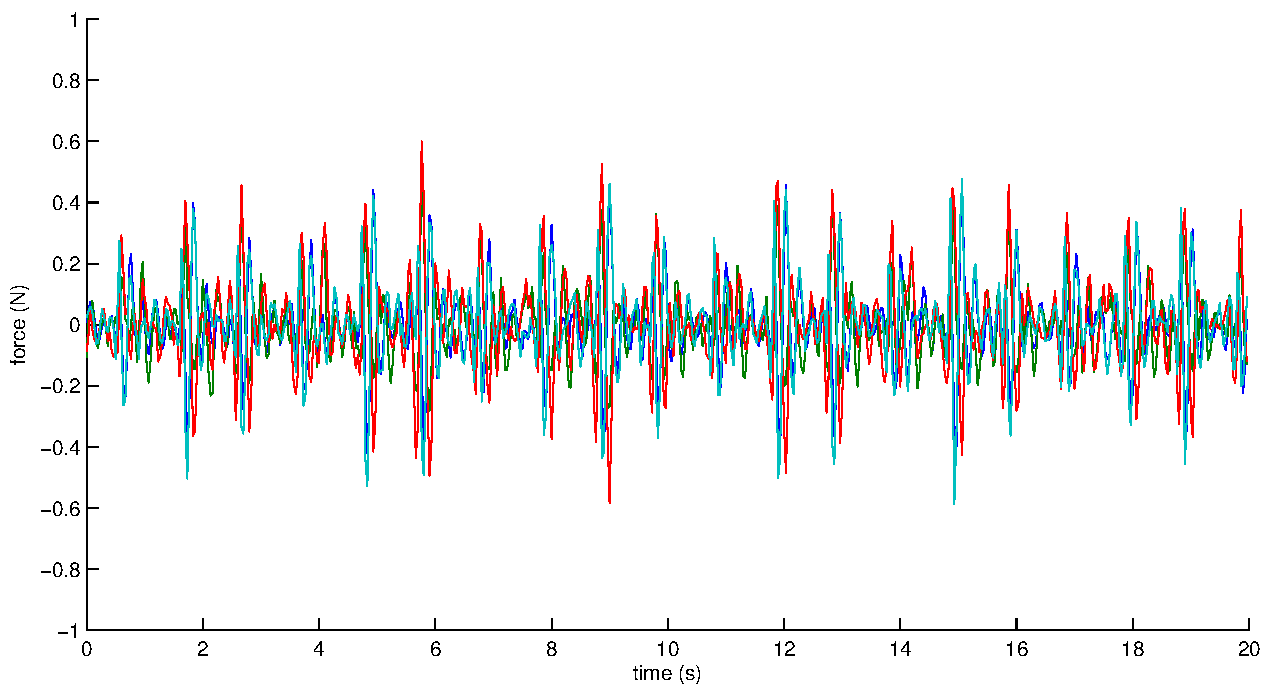
\includegraphics[width=0.8\columnwidth]{np1_data.pdf}} \\
\subfloat[Heartbeat timings from ECG (solid) and BCG (dashed) inferred by particle filter]{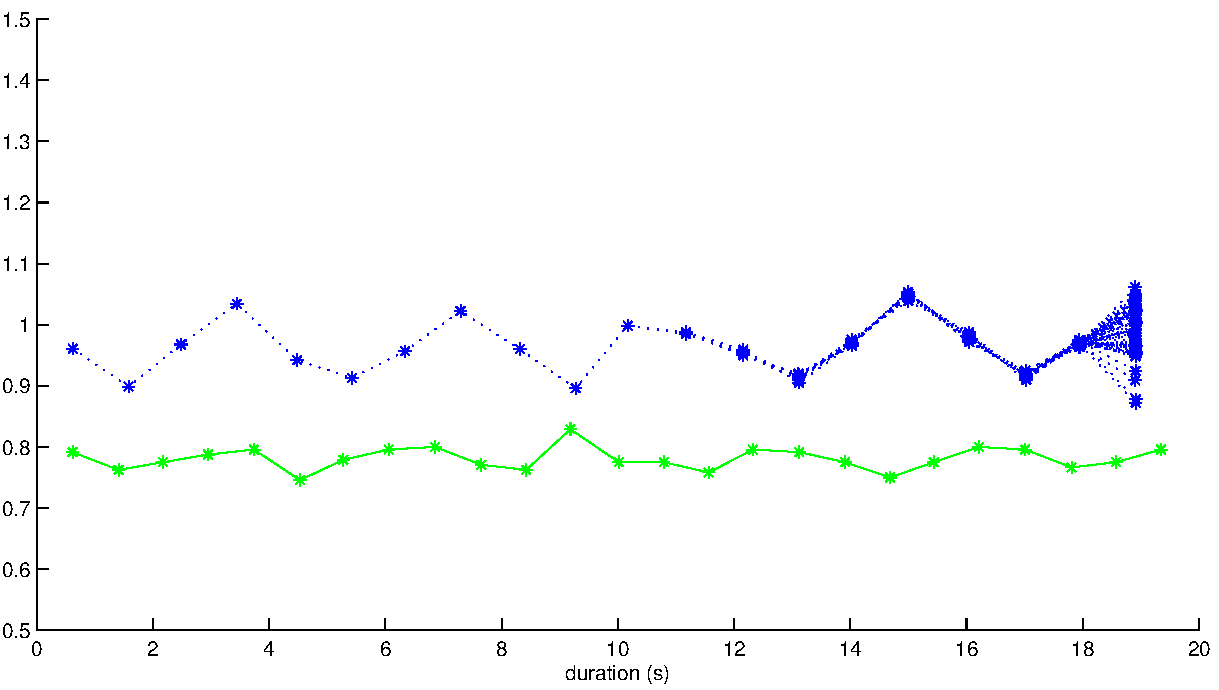
\includegraphics[width=0.8\columnwidth]{np1_timing.pdf}} \\
\subfloat[Particle filter effective sample size after each processing frame]{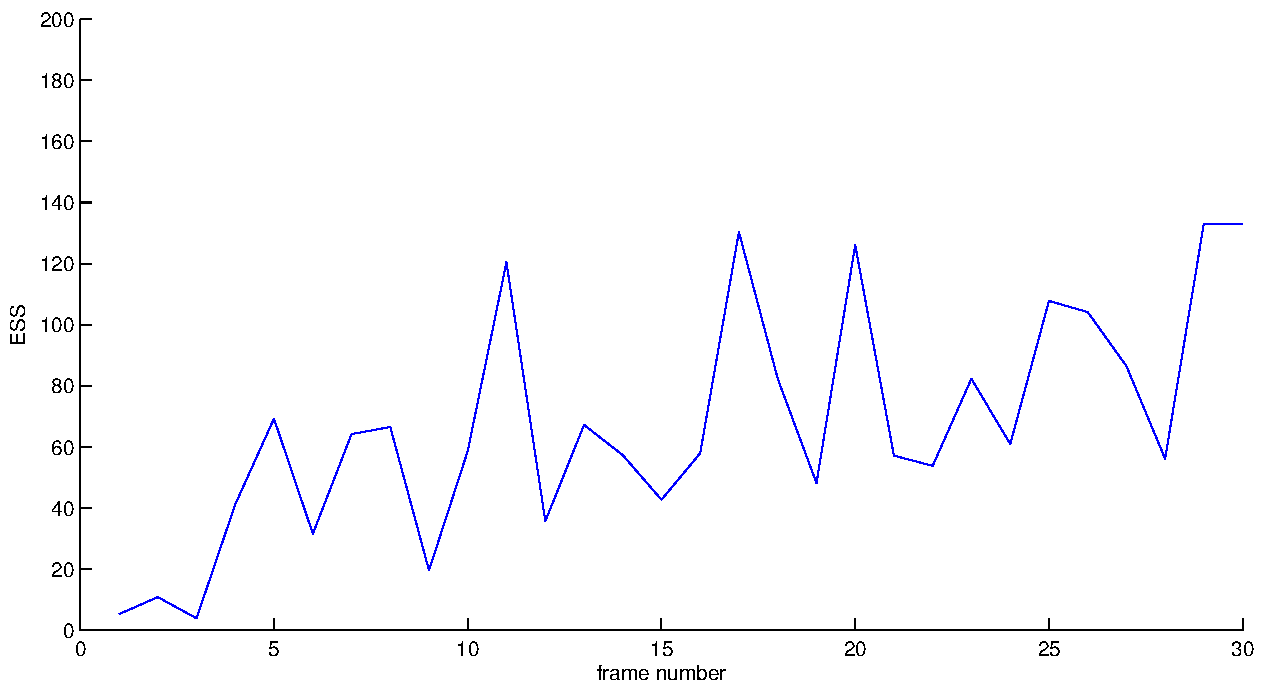
\includegraphics[width=0.8\columnwidth]{np1_ess.pdf}}
\caption{}
\label{fig:one_person}
\end{figure}

\begin{figure}
\centering
\subfloat[Measured force signal from sensors]{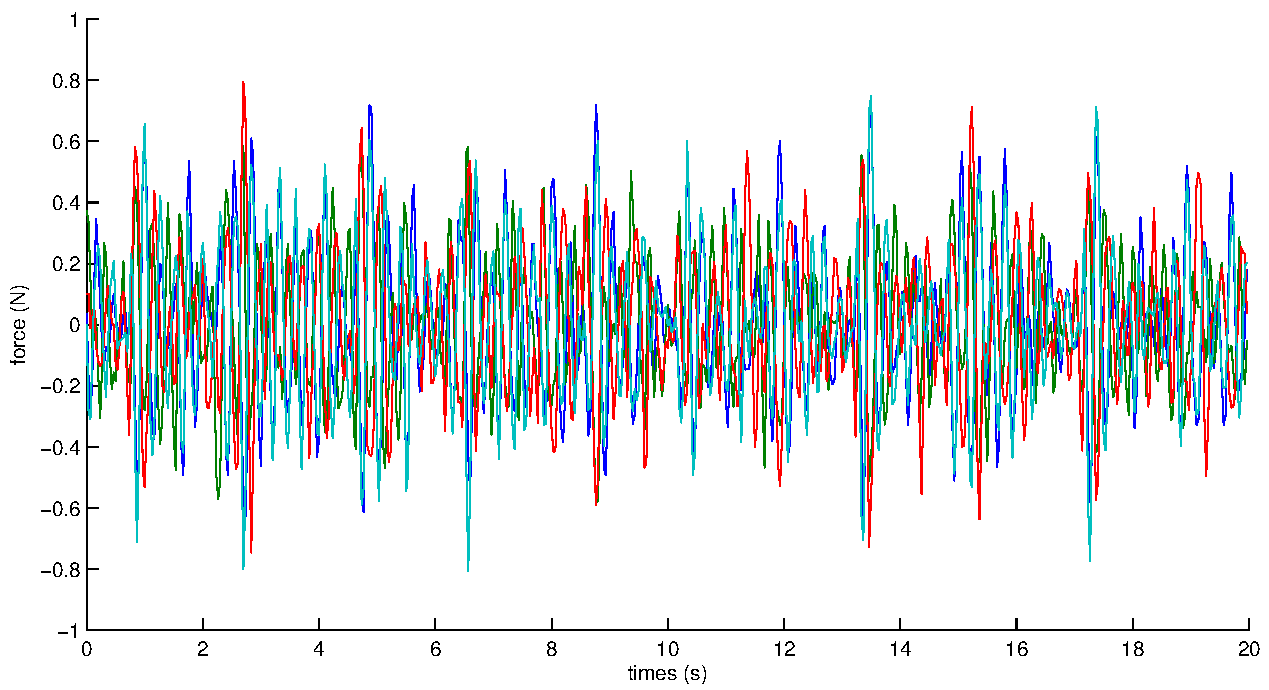
\includegraphics[width=0.8\columnwidth]{np2_data.pdf}} \\
\subfloat[Heartbeat timings from ECG (solid) and BCG (dashed) inferred by particle filter]{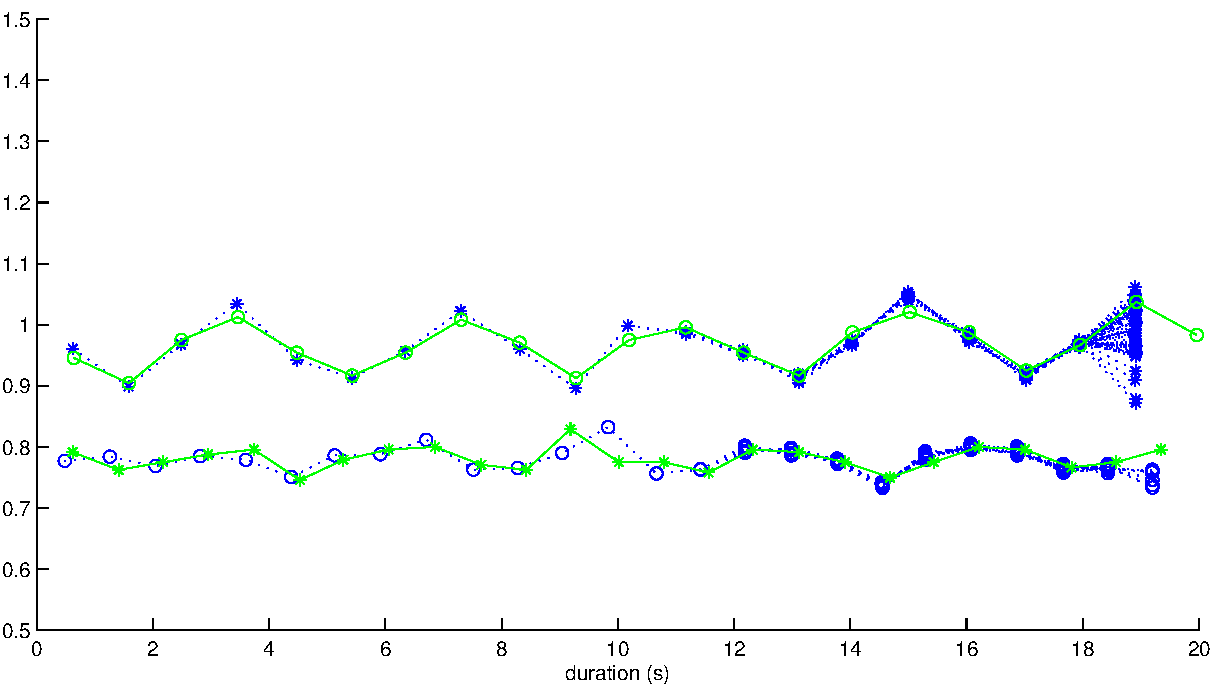
\includegraphics[width=0.8\columnwidth]{np2_timing.pdf}} \\
\subfloat[Particle filter effective sample size after each processing frame]{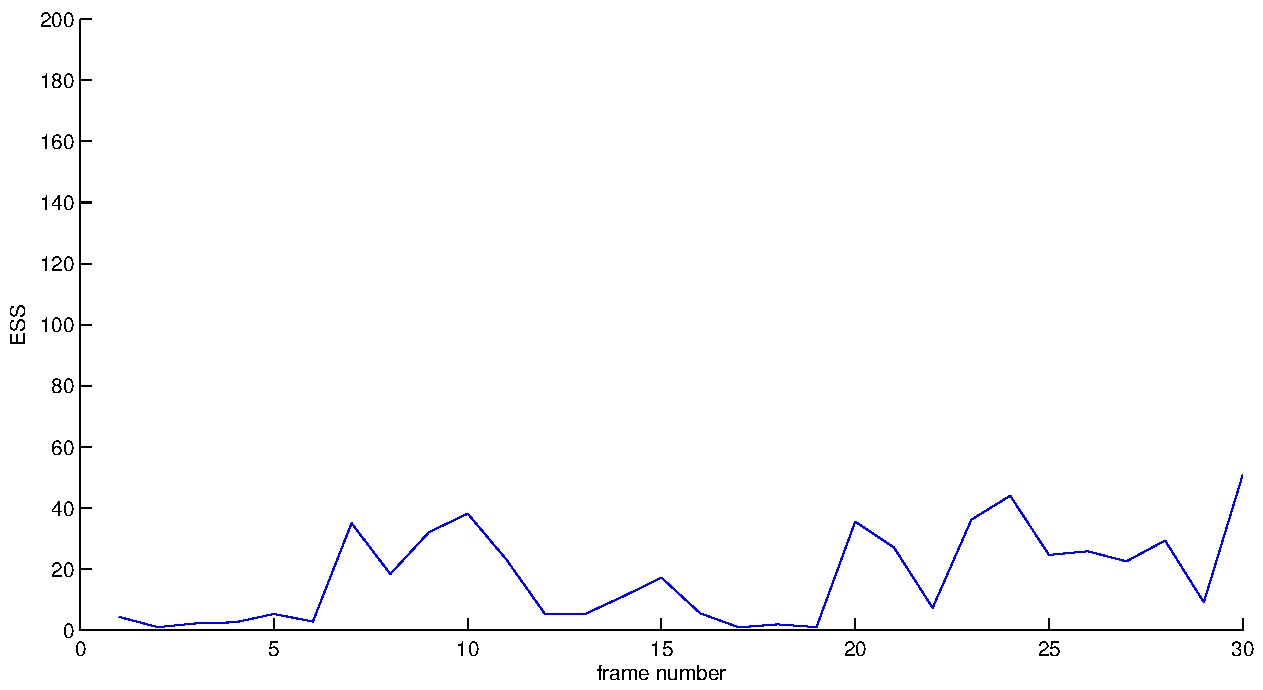
\includegraphics[width=0.8\columnwidth]{np2_ess.pdf}}
\caption{}
\label{fig:two_person}
\end{figure}

The algorithm was tested on eight data sets with each case (one- and two-person) with subjects lying in a variety of poses. In all cases, the inferred heartbeat times were in close agreement with those measured by the ECG. The effective sample sizes in the two-person case were very low, occasionally dropping to a single significant particle. At these points, all but one of the particle histories are discarded --- the algorithm is really producing a point estimate rather than a distribution. Effective sample sizes can be increased by decreasing the block length, $\blocklen$, at a proportional cost in computational time. A better design for the proposal mechanism may be required to alleviate this problem effectively.

\appendix

\section{Log-Likelihood Derivative for Linear-Gaussian Auxiliary Variable Model} \label{app:log-lhood-derivative}

Write the likelihood for the linear-Gaussian auxiliary variable model as a function of the sequence,
%
\begin{IEEEeqnarray}{rCl}
 \contlhood(\cp{\ti+\winlen}) & = & \lhood(\ob{\ti+1:\ti+\winlen} | \cp{\ti+\winlen}, \ob{1:\ti}) \nonumber \\
 & = & \int \normalden{\obwin}{\obsmatwin \transfunwin \cplpcat{\ti}}{\obscovwin} \normalden{\cplpcat{\ti}}{\cplptransmatwin{} \cplpmn{\ti}}{\cplptranscovwin{} + \cplptransmatwin{} \cplpvr{\ti} \cplptransmatwin{}^T} d\cplpcat{\ti} \nonumber \\
 & = & \normalden{\obwin}{\obsmatwin \transfunwin \cplptransmatwin{} \cplpmn{\ti}}{\obsmatwin \transfunwin \left( \cplptranscovwin{} + \cplptransmatwin{} \cplpvr{\ti} \cplptransmatwin{}^T \right) \transfunwin^T \obsmatwin^T + \obscovwin} \nonumber      ,
\end{IEEEeqnarray}
%
and the log-likelihood,
%
\begin{IEEEeqnarray}{rCl}
 \loglhood(\cp{\ti+\winlen}) & = & \log\left( \contlhood(\cp{\ti+\winlen}) \right) \nonumber      ,
\end{IEEEeqnarray}
%
where the various matrixes are defined in section~\ref{sec:lgav-likelihood-evaluation}. Now the derivative is obtained by,
%
\begin{IEEEeqnarray}{l}
 \frac{ \partial }{\partial \cpt[\sqi]{\cpi}} \normalden{\obwin}{\obsmatwin \transfunwin \cplpcat{\ti}}{\obscovwin} = \magdet{2 \pi \obscovwin}^{-\half} \frac{ \partial }{\partial \cpt[\sqi]{\cpi}} \exp\left\{ -\half \left(\obwin-\obsmatwin\transfunwin\cplpcat{\ti}\right)^T \obscovwin^{-1} \left(\obwin-\obsmatwin\transfunwin\cplpcat{\ti}\right) \right\} \nonumber \\
 \qquad = \magdet{2 \pi \obscovwin}^{-\half} \exp\left\{ -\half \left(\obwin-\obsmatwin\transfunwin\cplpcat{\ti}\right)^T \obscovwin^{-1} \left(\obwin-\obsmatwin\transfunwin\cplpcat{\ti}\right) \right\} \left[ \cplpcat{\ti}^T \frac{\partial\transfunwin^T}{\partial \cpt[\sqi]{\cpi}} \obsmatwin^T \obscovwin^{-1} \left(\obwin-\obsmatwin\transfunwin\cplpcat{\ti}\right) \right] \nonumber \\
 \qquad = \normalden{\obwin}{\obsmatwin \transfunwin \cplpcat{\ti}}{\obscovwin} \left[ \cplpcat{\ti}^T \frac{\partial\transfunwin^T}{\partial \cpt[\sqi]{\cpi}} \obsmatwin^T \obscovwin^{-1} \left(\obwin-\obsmatwin\transfunwin\cplpcat{\ti}\right) \right] \nonumber \\ \nonumber
\end{IEEEeqnarray}
%
\begin{IEEEeqnarray}{rCl}
 \frac{ \partial \contlhood }{\partial \cpt[\sqi]{\cpi}} & = & \int \left[\frac{ \partial }{\partial \cpt[\sqi]{\cpi}} \normalden{\obwin}{\obsmatwin \transfunwin \cplpcat{\ti}}{\obscovwin}\right] \normalden{\cplpcat{\ti}}{\cplptransmatwin{} \cplpmn{\ti}}{\cplptranscovwin{} + \cplptransmatwin{} \cplpvr{\ti} \cplptransmatwin{}^T} d\cplpcat{\ti} \nonumber \\
 & = & \int \normalden{\obwin}{\obsmatwin \transfunwin \cplpcat{\ti}}{\obscovwin} \normalden{\cplpcat{\ti}}{\cplptransmatwin{} \cplpmn{\ti}}{\cplptranscovwin{} + \cplptransmatwin{} \cplpvr{\ti} \cplptransmatwin{}^T} \left[ \cplpcat{\ti}^T \frac{\partial\transfunwin^T}{\partial \cpt[\sqi]{\cpi}} \obsmatwin^T \obscovwin^{-1} \left(\obwin-\obsmatwin\transfunwin\cplpcat{\ti}\right) \right] d\cplpcat{\ti} \nonumber \\
 & = & \contlhood(\cp{\ti+\winlen}) \int \normalden{\cplpcat{\ti}}{\cplpupdmnwin}{\cplpupdvrwin} \left[ \cplpcat{\ti}^T \frac{\partial\transfunwin^T}{\partial \cpt[\sqi]{\cpi}} \obsmatwin^T \obscovwin^{-1} \left(\obwin-\obsmatwin\transfunwin\cplpcat{\ti}\right) \right] d\cplpcat{\ti} \nonumber      ,
\end{IEEEeqnarray}
%
where
%
\begin{IEEEeqnarray}{rCl}
 \cplpupdvrwin & = & \cplppredvrwin - \cplppredvrwin \transfunwin^T \obsmatwin^T \left( \obscovwin + \obsmatwin \transfunwin \cplppredvrwin \transfunwin^T \obsmatwin^T \right)^{-1} \obsmatwin \transfunwin \cplppredvrwin \nonumber \\
 \cplpupdmnwin & = & \cplppredmnwin + \cplppredvrwin \transfunwin^T \obsmatwin^T \left( \obscovwin + \obsmatwin \transfunwin \cplppredvrwin \transfunwin^T \obsmatwin^T \right)^{-1} \left( \obwin - \obsmatwin \transfunwin \cplppredmnwin \right) \nonumber \\
 \cplppredvrwin & = & \cplptranscovwin{} + \cplptransmatwin{} \cplpvr{\ti} \cplptransmatwin{}^T \nonumber \\
 \cplppredmnwin & = & \cplptransmatwin{} \cplpmn{\ti} \nonumber       ,
\end{IEEEeqnarray}
%
in which only standard Gaussian identities have been used. Finally,
%
\begin{IEEEeqnarray}{rCl}
 \frac{ \partial \loglhood }{\partial \cpt[\sqi]{\cpi}} & = & \frac{1}{ \contlhood(\cp{\ti+\winlen}) } \frac{ \partial \contlhood }{\partial \cpt[\sqi]{\cpi}} \nonumber \\
 & = & \cplpupdmnwin^T \frac{\partial\transfunwin^T}{\partial \cpt[\sqi]{\cpi}} \obsmatwin^T \obscovwin^{-1} \left( \obwin - \obsmatwin \transfunwin \cplpupdmnwin \right) - \trace\left[ \transfunwin^{T} \obsmatwin^T \obscovwin^{-1} \frac{ \partial \transfunwin^T }{ \partial \cpt[\sqi]{\cpi} } \obsmatwin^T \cplpupdvrwin \right] \nonumber     ,
\end{IEEEeqnarray}
%
where standard Gaussian moment formulas are applied.



\bibliographystyle{dcu}
\bibliography{D:/pb404/Dropbox/PhD/Cleanbib}
\end{document} 